
In algorithm 2, we firstly convert $K$ partitions using standard TSP algorithm for each partition. In this stage, we used a different type of operation for cycles.

$Transfer2$ is the operation of transferring a node from the longest cycle to another edge of a shorter cycle.

\begin{figure}[h!]
\centering
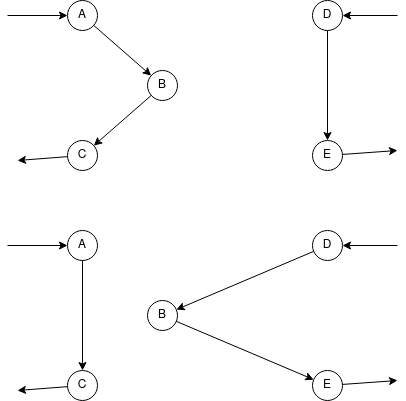
\includegraphics[width=0.8\textwidth]{assets/transfer2.png}
\caption{Transfer of $B$ to $D \to E$}
\label{fig:transfer2}
\end{figure}


\begin{algorithm}[H]
\caption{Local Search 2}
\label{algo:localsearch2}
\textbf{Input:}:

    Initial $K$ cycles
    
    Strategy $\in$ \{ first, best \} 

\textbf{Output:}:

    Final $K$ cycles
    
\textbf{Procedure:}:

While true:

    \hspace{1cm} var candidate\_set = []

    \hspace{1cm} For operation in all possible operations:
    
        \hspace{2cm} Calculate the gain of the operation
            
        \hspace{2cm} If operation reduced maximum cycle length and did not induce any intersection:
            
            \hspace{3cm} Push the operation and gain to candidate set
                
            \hspace{3cm} If Strategy is first:
                
                \hspace{4cm} break
                
    \hspace{1cm} If candidate\_set is empty:
    
        \hspace{2cm} break
    
    \hspace{1cm} Pick the candidate with smallest sum of cycle length, update the current $K$ partitions
    
return current $K$ partitions

\end{algorithm}